\subsection{Méthode RLE}

    La méthode RLE (Run-Length Encoding) est probablement la manière la plus simple pour un algorithme de compression sans perte. En effet, le principe est simple. Il suffit de compter le nombre d'occurence d'un caractère consécutifs, et d'encoder ce nombre d'occurence avec le caractère. La chaine de caractère \"aaaabbcbbb\" devient alors [(a,4), (b, 2), (c, 1), (b,3)].

    \medskip

    Cependant, cette méthode possède un assez gros défaut car elle ne peut pas compresser tout ce que l'on souhaite. Par exemple, il est très rare dans un texte qu'il y ait un grand nombre de caractères consécutifs. Lors de la compression, la sortie sera plus longue que l'entrée, ce qui n'est pas vraiment souhaitable. Par contre, il peut être assez efficace dans certains cas où il y a un grand nombre de données consécutives. Étudions ceci dans l'exemple suivant.

    \begin{figure}[H]
        \centering
        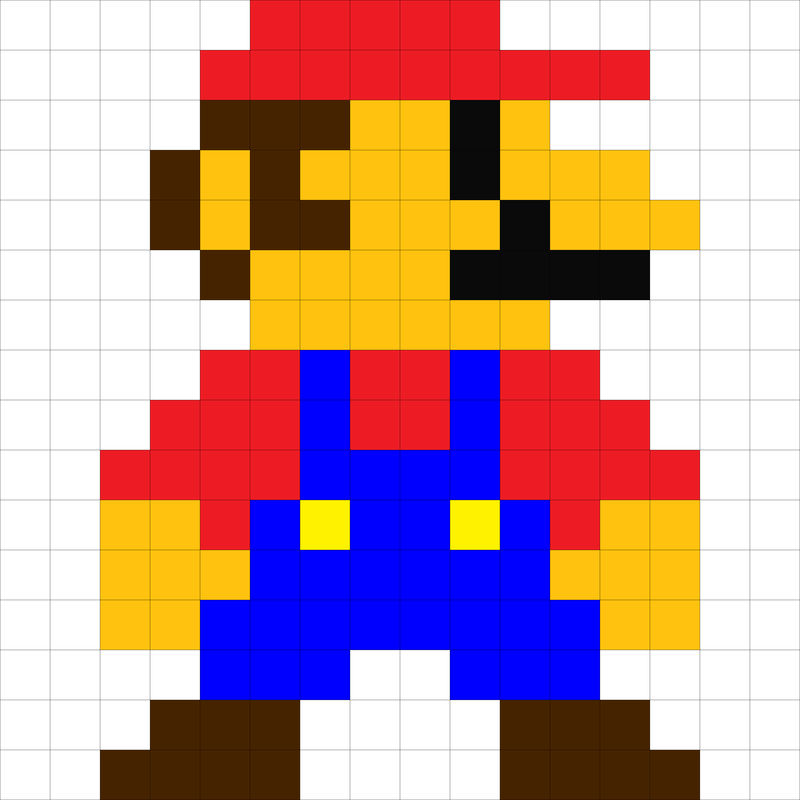
\includegraphics[width=0.5\linewidth]{assets/mario8bits.png}
        \caption{Mario 8-bits}
    \end{figure}

    Dans le cas du Mario en 8-bits, une représentation possible de l'encodage des bits pourrait être exprimée comme suit : [(5, blanc), (5, rouge), (10, blanc), \ldots]. Pour la première image, comprenant 256 pixels avec chaque pixel possédant 3 données (RGB), l'application de la compression RLE permet de réduire cela à seulement 75 changements de couleurs. Ainsi, la liste résultante a une longueur de 75, avec chaque élément comportant 4 données (le nombre de pixels identiques, RGB).

    \smallskip

    La première image a donc une taille de 768 bits, tandis que sa version compressée ne pèse plus que 300 bits. En conséquence, l'image compressée occupe environ 0.4 fois la taille de son équivalent initial.

